\chapter{Modellentwurf und Simulation}
Nach der sehr detaillreichen Analyse der Messwerte wird in diesem Kapitel ein Modell aus den aufbereiteten Daten gewonnen und dieses anschließend in eine Simulationsumgebung implementiert. Aus den Messungen muss zunächst qualitativ eine Aussage über das Verhalten der BLE-Signale getroffen werden, um nachfolgend ein geeignetes mathematisches Modell zu finden. Dieses gewählte Modell wird darauf an die Gegebenheiten mit einer Parameterschätzung angepasst. Für die Anpassung wird zunächst ein Minimierungsproblem anhand der Messwerte aus dem vorigen Kapitel erstellt, das mit einem Partikel-Schwarm-Optimierer gelöst wird. Die daraus gewonnenen Parameter lassen sich in die Modellgleichung einsetzen, um mit dessen Hilfe die Signalausbreitung der Beacons in einem Gebäude vorherzusagen. \\ \\
Die Prädiktion der Ausbreitung von BLE-Funkwellen in einer Simulation kann dazu genutzt werden, mithilfe eines Optimierungsverfahrens die Leuchtfeuer in einem Raum so anzubringen, dass ein Lokalisierungssystem aus dieser Technologie mit maximaler Genauigkeit konfiguriert werden kann. Um zuerst die Abmessungen des betreffenden Raumes zu ermitteln, wird der Grundriss durch die Verwendung des Scitos G5 und der Software Miracenter als Bilddatei erstellt. Somit gelten die Wände als Begrenzung und der verbleibende Raum als Platz für die Signalausbreitung. Die maximale Genauigkeit der Positionsbestimmung würde logischerweise erreicht werden, wenn der komplette Raum mit Beacons unter Einhaltung des Mindestabstandes übersäht wäre, was jedoch nicht ökonomisch ist. Deswegen wird zusätzlich die Anzahl der Beacons in die Problemformulierung eingearbeitet, sodass für jede mögliche Beacon-Anzahl eine optimale Konfiguration existiert. 
\section{Modellbildung}
\begin{table}[b!]
\begin{tabular}{|M{1.6cm}|M{1.9cm}|M{1.7cm}|M{1.6cm}|M{3.1cm}|M{3.1cm}|}
\hline 
Modell & Antennen-höhen & Frequenz & Bereich & In-/Outdoor & Bemerkungen \\ \hline 
Free Space Loss & nicht begrenzt & $f\geq$30 MHz & LOS begrenzt & Indoor-Indoor- bzw. Outdoor-Outdoor-Übertragungen bei direkter Sichtverbindung (LOS) & Systeme, bei denen direkte Sichtverbindung angenommen werden kann \\ \hline 
Extended Hata & $h_1=$[1 m ; 10 m] $h_2=$[30 m ; 100 m] & 30 MHz -- 3GHz & $d\leq40$ km & automatisches Hinzuaddieren von Verlusten an Wänden bei Indoor-Outdoor- bzw. Indoor-Indoor Übertragungen (mehrere Räume/Gebäude) & mobile und andere Dienste, ohne direkte Sichtverbindung, nur im Bereich 2 -- 3 GHz implementiert \\ \hline 
Extended Hata-SRD & $h=$[1,5 m ; 3 m] & 30 MHz -- 3GHz & $d\leq0,3$ km & automatisches Hinzuaddieren von Verlusten an Wänden bei Indoor-Outdoor- bzw. Indoor-Indoor Übertragungen (mehrere Räume/Gebäude) & Kurzstrecken-verbindungen, bei denen wenigstens LOS angenommen werden kann \\ \hline 
WINNER II & $h\leq6$ m & 2 GHz -- 6GHz & $d=$[5 m ; 100 m] & Indoor-Indoor-Übertragungen bei LOS oder NLOS & Anwendung in großen offenen Räumen bei hohem Datenverkehr (z.B. Konferenzhalle, Fabrikgebäude) \\ \hline 
\end{tabular} 
\caption{Übersicht der Kanalmodelle im Indoor-Bereich, in Anlehung an \cite{Kanal}}
\label{tab:Uebersicht}
\end{table}
Zunächst wird in diesem Abschnitt das zugrunde liegende Modell für das Verhalten der Signalausbreitung der Beacons bestimmt. Dazu wird aus Tabelle \ref{tab:Uebersicht} ein geeignetes Kanalmodell ausgesucht und dessen ungefährer Verlauf bestimmt. An diesem Verlauf wird es an den realen Messwerten validiert und anschließend in dessen Qualität durch die Parameterschätzung verbessert. Die genannten Modelle in der Tabelle können mit ihren Spezifikationen im Grunde alle als Ausbreitungsmodell für die Leuchtfeuer dienen. Jedoch fällt die erste Wahl auf das sogenannte WINNER II-Modell, weil in dessen Beschreibung die Anwendung in großen Räume mit hohem Aufkommen von Datenverkehr steht. Und weil diese Gegebenheiten in den Messungen aus dem vorigen Kapitel vorhanden sind und für den späteren Einsatzort (z.B. Kaufhäuser, Flugplätze etc.) der Beacon-Systeme gegeben sein müssen, ist dieses Modell vorzuziehen. Zudem beträgt die Reichweite eines Beacons nur 70 Meter, wohingegen die Geltungsbereiche der anderen Modelle dafür überdimensioniert erscheinen.
\subsection{Das WINNER II-Modell}
Das WINNER II-Modell \cite{WII} benannt nach dem "`Wireless-World-Initiative-New-Radio"' (WINNER)-Konsortium, das aus dem Zusammenschluss mehrerer Unternehmen besteht und die Verbesserung der Leistung von Mobilfunkkommunikationssystemen anstrebt, beinhaltet verschiedene Aspekte in der Berechnung von Ausbreitungsverlusten. Die Formel, die dem Modell zu Grunde liegt, beschreibt den Verlust einer Signalstärke in Abhängigkeit zu einem zurückgelegten Weg folgendermaßen:
\begin{align*}
L_{WINNER}\left [ dBm \right ]=A\cdot log_{10}\left (d\left [ m \right ]\right ) + B + C\cdot log_{10}\left (\frac{f_c\left [ GHz \right ]}{5}\right )
\end{align*}
In der Formel steht $L_{WINNER}$ für den Leistungspegel in Dezibel Milliwatt (dBm), der das logarithmische Verhältnis aus einer Leistung in Form der Empfangsstärke im Vergleich zur anfänglichen Sendeleistung des Beacons angibt. So kann die obige Gleichung umgeschrieben werden zu:
\begin{align*}
10\cdot log_{10}\left (\frac{P_{Sendung}\left [ mW \right ]}{P_{Empfang}\left [ mW \right ]}\right )=A\cdot log_{10}\left (d\left [ m \right ]\right ) + B + C\cdot log_{10}\left (\frac{f_c\left [ GHz \right ]}{5}\right )
\end{align*}
oder auch direkt als dBm-Einheit formuliert werden:
\begin{align}
L_{Sendung}\left [ dBm \right ] - L_{Empfang}\left [ dBm \right ]=A\cdot log_{10}\left (d\left [ m \right ]\right ) + B + C\cdot log_{10}\left (\frac{f_c\left [ GHz \right ]}{5}\right ) \label{eq:WII}
\end{align}
Die Parameter der Gleichung bestehen primär aus einem Koeffizienten $A$, der die in der Luft zurückgelegte Strecke des Signals proportional gewichtet. Des Weiteren fließen zum einen noch der additive Einfluss von dem Parameter $B$ für sonstige Störfaktoren und zum anderen der ebenfalls multiplikative Faktor $C$ zur Gewichtung des Ausbreitungsverlustes durch die Frequenz $f_c$ mit ein. In Abbildung \ref{fig:QualiWII} ist der qualitative Verlauf der Empfangsstärke, die nach oben hin abnimmt und der Distanz, die nach rechts zunimmt, skizziert. Als Parameter wurden Werte aus der Fachliteratur \cite{Kanal} entnommen und in die Gleichung eingesetzt. Im Vergleich zu Abbildung \ref{fig:Mittelwert100} sieht der Funktionsverlauf weitgehend identisch aus, sodass nun mit der Parameterschätzung begonnen werden kann.  
\begin{figure}[H]
\centering
\begin{tikzpicture}
\begin{axis}[ymax=-40, xlabel={Distanz}, ylabel={Empfangsstärke}, width=0.5\paperwidth, height=0.2\paperheight, xtick = \empty, y dir=reverse, ytick = \empty, axis y line = left, axis x line = bottom, axis line style = {-latex}]
\addplot[domain=0.5:15, samples=100]{-(13.9*ln(x)+64.4+20*ln(2.4/5)+12)};
\end{axis}
\end{tikzpicture}
\caption{Qualitativer Verlauf des WINNER II-Modells}
\label{fig:QualiWII}
\end{figure}
\subsection{Parameterschätzung}
Um die qualitative Repräsentation des WINNER II-Modells in eine qualitative für die Beschreibung des Ausbreitungsverlustes von BLE-Signalen zu überführen, müssen die Parameter $A$, $B$ und $C$ dementsprechend angepasst werden. Die Gleichung aus \ref{eq:WII} vereinfacht sich dabei nochmals, wenn $f_c$ als konstant angenommen wird und die Ausdrücke aus $B$ und $C$ miteinander zu dem neuen Parameter $B^{\ast}$ zusammengefasst werden. Die Anpassung wird dabei in Form einer Optimierungsaufgabe vorgenommen, wobei es gilt, die richtige Distanz anhand der RSSI-Werte zu schätzen. Im vorangegangenen Kapitel ergaben die Messungen, dass unter Betrachtung aller Daten es sehr schwierig ist eine genaue Vorhersage zu treffen. Deswegen wurden nur die stärksten 100 Signale einer Distanz gemittelt und diese Ergebnisse unter Abb. \ref{fig:Mittelwert100} vorgestellt. Die Durchschnittswerte werden anschließend zusammen mit den realen Distanzen in gleicher Reihenfolge der Länge $k$ in die zwei Vektoren $d_{real}\left ( k \right )$ und $RSSI\left ( k \right )$ gespeichert. Aus der Umstellung der Gleichung \ref{eq:WII} nach $d$ lässt sich aus dem empfangenen RSSI-Wert die geschätzte Entfernung bestimmen. Mit all diesen Informationen lässt sich ein Optimierungsproblem so formulieren, dass eine zu minimierende Kostenfunktion $J$ als Differenz aus der direkt gemessenen Distanz eines Beacons zum Smartphone zu der berechneten Distanz aufgefasst und durch deren folgende Quadrierung so eine parabolische Funktion erstellt wird. Die Quadrierung bewirkt, dass der Wert der Kostenfunktion von allen Seiten in Richtung des globalen Minimums abnimmt und somit das Optimierungsproblem einfacher zu lösen ist. 
\begin{align}
\underset{A,B^{\ast}}{min}\, J=\sum_{k=1}^{k_{end}}\left ( d_{real}\left ( k \right ) -10^{\frac{L_{Sendung} - RSSI\left ( k \right ) - B^{\ast}}{A}} \right )^{2} \label{eq:WIIOpti}
\end{align}
Als Lösungsalgorithmus für die Optimierung wird ein Partikel-Schwarm-Algorithmus (PSO) gewählt. Der Partikel-Schwarm-Optimierer ist ein Algorithmus mit einer künstlichen Intelligenz, die es zur Aufgabe hat, eine Funktion zu minimieren bzw. zu maximieren. Es ist dabei einfacher, sich die Partikel als einen Vogelschwarm vorzustellen. Der Grundgedanke dabei ist, dass mehreren Partikeln ein zufälliger Startwert $p\left( t \right)$ im Suchraum unter Berücksichtigung der Gleichungsnebenbedingungen zugeordnet wird. D.h. im übertragenen Sinn, dass ein Vogelschwarm auf einer Wiese ausgesetzt wird. Ausgehend von diesem Startwert werden die einzelnen Vögel/Partikel im ersten Schritt in verschiedene Richtungen mit unterschiedlichen Geschwindigkeiten geschickt. Anschließend werden an den Zielpunkten die Kostenfunktionen mit den Positionen (oder auch Parametersätzen) berechnet und so der Funktionswert bestimmt. Die Schwarmintelligenz wird hierbei so realisiert, dass jedes Individuum seine aktuelle Position mit den zugehörigen Kosten kennt sowie über die Position des Partikels mit den geringsten Kosten im ganzen Schwarm informiert wird. In Folge des Wissens um die beste Position, fliegen alle Vögel/Partikel in Richtung des lokalen Minimum und decken somit den gesamten Raum ab. \\ \\
Als Gleichung aufgefasst wird die Geschwindigkeit $v$ im nächsten Zeitschritt $t+1$ eines Partikels aus der alten Geschwindigkeit $v\left( t \right)$, aus den drei konstanten Gewichtungen $w$, $r_1$ und $r_2$, zwei Zufallszahlen $c_1$ und $c_2$ und verschiedenen Positionen berechnet. Die Punkte sind zum einen die aktuelle Position $x\left( t \right)$, die mit den besten Kosten des einzelnden Individuums $p$ und zum anderen die Generation der geringsten Kosten im ganzen Schwarm $g$. Im Ganzen lauten die Gleichungen zur Bestimmung des nächsten Punktes \cite{PSO}:
\begin{align}
v\left( t+1 \right)&=w\cdot v\left( t \right) + c_1\cdot r_1\cdot \left( p - x\left( t \right) \right)+c_2\cdot r_2\cdot \left( g - x\left( t \right) \right) \\
x\left( t+1 \right)&=x\left( t \right) + v\left( t+1 \right)
\end{align}
Das Abbruchkriterium wird hierbei mit einer maximalen Anzahl an Generationen/Durchläufen der Hauptschleife angegeben. Der Vorteil dieses Verfahrens ist es, dass der komplette Suchraum abgetastet wird und durch die Intelligenz des Schwarms die Parametersätze mit den geringsten Kosten identifiziert werden. Der Nachteil ist der relativ hohe Rechenaufwand im Gegensatz zu anderen Verfahren (z.B. Newton, Trust-Region, Simplex etc.), zumal kein besseres Ergebnis mit dem PSO für ein solches Problem zu erwarten wäre. Jedoch baut der erweiterte Partikel-Schwarm-Optimierer in einem der nächsten Abschnitte auf diesem Verfahren auf, sodass in diesem Teil der Arbeit die Vorstellung der einfachen Variante zur Einführung vorteilig ist.\\ \\
Als Ergebnis der Parameterschätzung wurden in Abbildung \ref{fig:WIISauelengraph} zunächst die berechneten RSSI-Werte für die jeweiligen Distanzen im Vergleich zu den gemessenen Mittelwerten aller drei Beacons gegenübergestellt. Wie schon in der Analyse der Messwerte kritisiert, entspricht das Verhalten des Ausbreitungsverlustes ab dem zehnten Meter nicht mehr der theoretischen Annahme. Während der Verlauf vom ersten Abschnitt sehr gut geschätzt werden kann, versagt aber das einfache WINNER II-Modell bei größeren Distanzen. Ähnlich verhält es sich bei der Schätzung der Entfernung, wie Abbildung \ref{fig:WIIDistance} zeigt. Hier wurde das Modell lediglich nach $d$ umgestellt und als Eingabe dienten die Mittelwerte aus \ref{fig:WIISauelengraph}. In Tabelle \ref{tab:Parameterwerte} sind die Parameter aus der Optimierung aufgeführt, welche in das Modell zur Berechnung der letzten Diagramme eingesetzt wurden. 
\begin{figure}[H] 
\centering
\begin{tikzpicture}
\begin{axis}[ybar, bar width=1.5mm, xlabel={Abstand der einzelnen Beacons in Metern}, ylabel={Gemittelter RSSI-Wert in dBm}, width=0.7\paperwidth, height=0.2\paperheight, y dir=reverse, legend style={at={(0.25,1.15)}, anchor=south, legend columns=5, /tikz/every even column/.append style={column sep=0.2cm}}, enlarge y limits=false, enlarge x limits=false, ymin=-90,ymax=-60, xmin=0.3,xmax=15.7]
\addplot+[fill=dblue] table [col sep=comma] {TikzDaten/WIISauelengraph.dat}; 
\legend{Mittelwert aller drei Beacons}
\end{axis}
\begin{axis}[xtick = \empty, ytick = \empty, width=0.7\paperwidth, height=0.2\paperheight, y dir=reverse, legend style={at={(0.75,1.15)}, anchor=south, legend columns=5, /tikz/every even column/.append style={column sep=0.2cm}}, enlarge y limits=false, enlarge x limits=false, ymin=-90,ymax=-60, xmin=0.3,xmax=15.7]
\addplot+[mark=none,red,very thick] table [col sep=comma] {TikzDaten/WIIRSSI.dat};
\legend{geschätzter RSSI-Wert};
\end{axis}
\end{tikzpicture}
\caption{Durschnittlicher RSSI-Wert und berechneter RSSI-Wert im Vergleich}
\label{fig:WIISauelengraph}
\end{figure}
\begin{table}[H]
\begin{center}
\begin{tabular}{|c|c|c|}
\cline{2-3}
\multicolumn{1}{c|}{} & \multicolumn{2}{c|}{Parameter} \\
\cline{2-3}
\multicolumn{1}{c|}{} & $A$ & $B^{\ast}$ \\
\hline
\multirow{1}{*}{Wert} & $16,2623$ & $55,1046$ \\
\hline
\end{tabular}
\end{center}
\caption{Parameter des Modells}
\label{tab:Parameterwerte}
\end{table} 
\begin{figure}[H] 
\centering
\begin{tikzpicture}
\begin{axis}[xlabel={Reale Distanz in Meter},ylabel={Geschätzte Distanz in Meter},width=0.7\paperwidth, height=0.25\paperheight, enlarge y limits=0.01, enlarge x limits=false, xmin=0.3,xmax=15.7, legend pos=north west]
\addplot+[red,mark=*,semithick] table [col sep=comma] {TikzDaten/WIIdberech.dat}; 
\addplot+[mark=none,blue,very thick] table [col sep=comma] {TikzDaten/DisrealOptimum.dat};
\legend{geschätzter Wert,optimaler Verlauf};
\end{axis}
\end{tikzpicture}
\caption{Vergleich der Distanz-Schätzung mit dem WINNER II-Modell zur gemessenen Entfernung}
\label{fig:WIIDistance}
\end{figure}
\section{Vertrauensskala}
Im Hinblick auf die verschiedenen Betriebsmodi der Beacons, den unterschiedlichen Arten der Positionsbestimmung (Landmarkensystem und Mikro-Lokalisierung) und vielen noch nicht vorgestellten Techniken mit denen sich die Vorhersage der Position bestimmen und verbessern lassen, fällt es sehr schwer die Güte der Leuchtfeuer-Signale einzuschätzen. Mit Güte ist gemeint, inwieweit dem Modell \ref{eq:WII} vertraut wird die aktuelle Position zu schätzen und wie genau diese Schätzung in Metern oder Zentimetern erfasst werden kann. Um unabhängig von der Art der Lokalisierung, dem Anwendungsbereich und den eingesetzten Techniken die Güte angeben zu können, wird lediglich die Wahrscheinlichkeit mit dem WINNER II-Modell die tatsächliche Distanz zu ermitteln, als Wert dafür angenommen. D.h. aus den Messungen der RSSI-Werte vom vorigen Kapitel werden dieses Mal alle Daten für die Distanzberechnung herangezogen und mit einer Toleranz versehen. Die berechneten Entfernungen werden daraufhin mit realen Distanzen verglichen und im Falle, dass sie sich nur in einem definierten Spielraum voneinander unterscheiden, wird dies als eine erfolgreiche Positionsbestimmung angesehen. Der prozentuale Anteil aller erfolgreichen Berechnungen wird so als Gütemaß gewertet und somit ist die Qualität der Beacon-Signale als eine statistische Wahrscheinlichkeit, des Empfanges einer für das Modell geeigneten Signalsstärke pro Messung, aufzufassen. Die Ergebnisse aus diesen Überlegungen finden sich in Abbildung \ref{fig:GueteSauelengraph05} und \ref{fig:GueteSauelengraph2} wieder. Sie zeigen einmal die Wahrscheinlichkeit $W_{berech}$ ein gültiges Signal zu empfangen bei einer Toleranz von $0,5$ und bei $2$ Metern, wobei die dazugehörigen festen Distanzen die jeweiligen gemittelten drei Messreihen $d_{mitt}$ darstellen. Zudem wurde versucht, die Güte als Funktion zu charakterisieren. Dazu wurde die Funktion \ref{eq:Umkehrfunktion} aufgrund ihrer Art ausgewählt und um weitere Parameter erweitert (siehe Gleichung \ref{eq:eUmkehrfunktion}), die schließlich durch die Lösung des Minimierungsproblems unter \ref{eq:OptiUmkehrfunktion} und unter der Verwendung vom PSO bestimmt wurden (Ergebnis siehe Tabelle \ref{tab:ParameterwerteGuete}).
\begin{align}
W_{berech}&=\frac{1}{d_{mitt}+1} \label{eq:Umkehrfunktion}\\
W_{berech}&=\frac{1}{p_1\cdot d_{mitt}+p_2} + p_3 \label{eq:eUmkehrfunktion}\\
\underset{p_1,p_2,p_3}{min}\, J&=\sum_{k=1}^{k=15}\left ( W_{real}\left ( k \right ) - W_{berech} \right )^{2} \label{eq:OptiUmkehrfunktion}
\end{align}
Der Vorteil dieser Betrachtungsweise liegt in den Funktionen der Beacons begründet, da hier die Frequenz bzw. Häufigkeit der Sendevorgänge eingestellt werden kann. Durch die Erhöhung der Übertragungen pro Sekunde lässt sich somit die Zeit verringern, bis ein gültiges Signal das Messgerät erreicht. Anhand dieser Einstellmöglichkeiten lässt sich zusammen mit der hier vorgestellten Skala die Dynamik der Messungen beeinflussen. 
\begin{figure}[H] 
\centering
\begin{tikzpicture}
\begin{axis}[ybar, bar width=1.5mm, xlabel={Abstand der einzelnen Beacons in Metern}, ylabel={Wahrscheinlichkeit}, width=0.7\paperwidth, height=0.2\paperheight, legend style={at={(0.25,1.15)}, anchor=south, legend columns=5, /tikz/every even column/.append style={column sep=0.2cm}}, enlarge y limits=false, enlarge x limits=false, ymin=0,ymax=1, xmin=0.3,xmax=15.7]
\addplot+[fill=dblue] table [col sep=comma] {TikzDaten/GueteSauelengraph05.dat}; 
\legend{gemessener Durschnittswert}
\end{axis}
\begin{axis}[xtick = \empty, ytick = \empty, width=0.7\paperwidth, height=0.2\paperheight, legend style={at={(0.75,1.15)}, anchor=south, legend columns=5, /tikz/every even column/.append style={column sep=0.2cm}}, enlarge y limits=false, enlarge x limits=false, ymin=0,ymax=1, xmin=0.3,xmax=15.7]
\addplot+[mark=none,red,very thick] table [col sep=comma] {TikzDaten/GueteOpit05.dat};
\legend{Approximation};
\end{axis}
\end{tikzpicture}
\caption{Wahrscheinlichkeit des Empfangs gültiger Signale in einem Toleranzbereich von $0,5$ Meter und dessen Approximation}
\label{fig:GueteSauelengraph05}
\end{figure} 
\begin{figure}[H] 
\centering
\begin{tikzpicture}
\begin{axis}[ybar, bar width=1.5mm, xlabel={Abstand der einzelnen Beacons in Metern}, ylabel={Wahrscheinlichkeit}, width=0.7\paperwidth, height=0.2\paperheight, legend style={at={(0.25,1.15)}, anchor=south, legend columns=5, /tikz/every even column/.append style={column sep=0.2cm}}, enlarge y limits=false, enlarge x limits=false, ymin=0,ymax=1, xmin=0.3,xmax=15.7]
\addplot+[fill=dblue] table [col sep=comma] {TikzDaten/GueteSauelengraph2.dat}; 
\legend{gemessener Durschnittswert}
\end{axis}
\begin{axis}[xtick = \empty, ytick = \empty, width=0.7\paperwidth, height=0.2\paperheight, legend style={at={(0.75,1.15)}, anchor=south, legend columns=5, /tikz/every even column/.append style={column sep=0.2cm}}, enlarge y limits=false, enlarge x limits=false, ymin=0,ymax=1, xmin=0.3,xmax=15.7]
\addplot+[mark=none,red,very thick] table [col sep=comma] {TikzDaten/GueteOpit2.dat};
\legend{Approximation};
\end{axis}
\end{tikzpicture}
\caption{Wahrscheinlichkeit des Empfangs gültiger Signale in einem Toleranzbereich von $2$ Metern und dessen Approximation}
\label{fig:GueteSauelengraph2}
\end{figure} 
\begin{table}[H]
\begin{center}
\begin{tabular}{|c|c|c|c|c|}
\cline{3-5}
\multicolumn{2}{c|}{} & \multicolumn{3}{c|}{Parameter} \\
\cline{3-5}
\multicolumn{2}{c|}{} & $p_1$ & $p_2$ & $p_3$ \\
\hline
\multirow{2}{*}{Toleranz} & $0,5$ m & $3,3777$ & $-0,6746$ & $0.0163$\\
\cline{2-5}
& $2$ m & $0,2035$ & $0,7145$ & $0,1594$\\
\hline
\end{tabular}
\end{center}
\caption{Parameter der Vertrauensskala}
\label{tab:ParameterwerteGuete}
\end{table} 
\section{Entwicklung der Simulationsumgebung}
Mit den gewonnen Erkenntnissen aus der Modellbildung können nun Vorhersagen über die Signalausbreitung und der zu erwartenden Genauigkeit der Entfernungsschätzungen getroffen werden, die schließlich zu einer optimalen Planung eines Indoor-Lokalisierungssystems genutzt werden können. Dazu wird zunächst eine Entwicklungsumgebung zur Herstellung der Simulation benötigt. Als Basis der Simulation wird eine grafische Oberfläche (GUI) mit dem Editor GUIDE erstellt, der Teil des Programmes MATLAB \cite{GUIDE} ist. In dieser Sektion werden die einzelnen Funktionen der GUI besprochen und deren Verarbeitungskette vorgestellt. Hierfür wird als erstes die Konvertierung der Zeichnung eines Grundrisses (als PNG-Bilddatei) in verarbeitbare Informationen erläutert, die von substantieller Bedeutung für den gesamten Simulationsprozess ist. Anschließend wird in der weiteren Implementierung speziell der Aspekt einer optimalen Verteilung, unter besonderer Betrachtung der Vertrauensskala, aufgegriffen. Eigens dafür wurde der vorher vorgestellte Partikel-Schwarm-Algorithmus aus der Parameterschätzung erweitert, sodass er auch für den abstrakten Fall einer Anordnung von Funkbaken eingesetzt werden kann. Abschließend wird mit einem fiktiven Grundriss das komplette Lighthouse Keeper-Prinzip exemplarisch vorgeführt.  
\subsection{Grundrissanalyse}
Für eine weitgehende Automation der gesamten Planung müssen die Grundrisse bzw. Rauminformationen, die mit der Software Miracenter (siehe Abschnitt \ref{sec:Mira}) generiert wurden, vor der Simulation ausgewertet werden. In der Auswertung oder Analyse dieser Daten muss das Programm selbstständig in der Lage sein, eine Wand oder generell einen Raum zu erkennen. Zudem müssen auch Befestigungspunkte definiert sein, an denen die Beacons angebracht werden können. Die Umsetzung dieser Funktionen basiert hierbei auf einer Eigenentwicklung, da bisher keine vergleichbaren Arbeiten existieren. Für die Erkennung von Wänden respektiven Räumen könnten zwar Algorithmen eingesetzt werden, die beispielsweise Formen erkennen oder Cluster von Farbgruppierungen bilden. Im Hinblick jedoch auf mögliche Erweiterungen der gesamten Problematik, z.B. mit Hindernissen oder mit Bereichen, in denen keine Beacons befestigt werden können, bietet sich das hier selbstentwickelte Verfahren an. Für ein besseres Verständnis wird der allgemeine Vorgang diesbezüglich in Abbildung \ref{fig:GrundAna} illustriert. Das Beispiel zeigt einen quadratischen Raum, wobei die Wände in schwarz und die freien Räume in weiß gehalten sind. Die einzelnen Unterteilungen sollen die Pixel darstellen, sodass eine Auflösung von 7 $\times$ 7 Pixeln gegeben ist. In einer ersten Phase werden in vertikaler Reihenfolge die einzelnen Pixel von "`links nach rechts"' sowie deren Vorgängerpixel und deren Nachfolgerpixel betrachtet. Im vorliegenden Fall werden dafür zwei Matrizen mit 7 $\times$ 7 Einträgen initialisiert, in der jeder Eintrag zunächst auf Null gesetzt ist. Wechselt in der abgefragten Reihe ein weißer Pixel auf einen schwarzen, so wird die Position des schwarzen Pixels in der Befestigungs-Matrix um eins erhöht und in der Raum-Matrix wird die Position des weißen Pixels ebenfalls mit eins addiert. Die folgenden weißen Pixel werden anschließend auch als Raumkoordinaten markiert, solange kein weiterer schwarzer Punkt erscheint. Falls eine weitere Wand im Verlauf der Reihe detektiert wird, setzt die Raummarkierung aus und lediglich der schwarze Bildpunkt wird als Befestigung eingeschrieben. \\ \\
Diese Vorgehensweise allein ist jedoch nicht robust genug, was auch in der Abbildung skizziert wurde. In diesem Fall wurden zwei Befestigungen und zwei Raumpunkte falsch interpretiert, weil der Algorithmus nur den unmittelbaren Nachbarn eines Bildpunktes betrachtet und somit nicht feststellen konnte, ob der Raum mit Wänden komplett umschlossen ist oder nicht. In Folge dieses bekannten Fehlers wurde für alle weißen Pixelkoordinaten an den Bild-Rändern eine rückwärtsgerichtete Suche implementiert, die bis zur nächsten Wand alle Einträge beider Matrizen um eins reduziert, wie auch rechts neben der ersten Phase zu sehen ist. Somit wird sichergestellt, dass die Räume stets abgeschlossen sind und keine Befestigungen an den Ecken existieren. Die gleiche Vorgehensweise wird dreimal in jede Richtung ("`von rechts nach links"', "`von unten nach oben"' und "`von oben nach unten"') wiederholt. Dabei entstehen Vertrauenswerte in den Matrizen, anhand derer über die endgültige Definition nach Befetigungen und Räumen entschieden wird. In den verschiedenen Versuchen und Testszenarien mit offenen Türen und verwinkelten Gängen erwies sich der vorgestellte Algorithmus als sehr zuverlässig. Zusätzlich wurde die Analyse auf den Rot-, Grün- und Blau-Farbraum (RGB) erweitert, sodass mit weiteren Farben spezielle Objekte erfasst werden. Zum Beispiel können nun mit roten Farben Bereiche gekennzeichnet werden, an denen keine Beacons befestigt werden können. \\ \\
Damit die Bildinformationen im metrischen Raum abgebildet werden können, muss zunächst deren Verhältnis von Pixel zu Meter bekannt sein. In der Simulation kann dieses Verhältnis direkt angegeben werden, indem die Abmessungen des gesamten Raumes in die GUI eingetragen werden. Aus diesen Informationen berechnet die Software eigenständig die Verhältnisse und überträgt die Pixel in metrische Koordinaten. Anschließend werden die Wände bzw. Befestigungen durch einfache Polygone ersetzt, wobei die Ecken von Wänden als Referenzpunkte genommen werden. Dies hat den Vorteil, dass für eine Aufteilung der Beacons entlang dieser Linien nur Abstandswerte kalkuliert werden müssen. Zudem kann die Kollision von Signalen und Wänden schneller berechnet und somit entschieden werden, ob sich ein Beacon in der LOS oder NLOS zu einem Punkt im Raum befindet. Im letzten Schritt der Analyse wird der Raum in einzelne Elemente untergliedert. Die Größe der Quadrate wird dazu in die Oberfläche der Simulation eingetragen. Die Aufteilung in finite Elemente ergibt sich aus der Nutzung der Vertrauensskala, die abhängig von der gewünschten Toleranz bzw. Lokalisierungsgenauigkeit ist. Diese Toleranz bildet die Größe eines Raumelementes, in der die modellbasierte Entfernungsschätzung ($\pm$ der Toleranz) mit einer bestimmten Wahrscheinlichkeit den tatsächlichen Abstand eines Raumelementes zu einem Beacon angibt. \\ \\
\def\x{0.8}
\begin{figure}[H] 
\centering
\begin{tikzpicture}
\fill[black, draw=gray] (1*\x,11*\x) rectangle (2*\x,12*\x);
\fill[black, draw=gray] (2*\x,11*\x) rectangle (3*\x,12*\x);
\fill[black, draw=gray] (3*\x,11*\x) rectangle (4*\x,12*\x);
\fill[black, draw=gray] (4*\x,11*\x) rectangle (5*\x,12*\x);
\fill[black, draw=gray] (5*\x,11*\x) rectangle (6*\x,12*\x) node[pos=.5, text=white] {$1$};

\fill[black, draw=gray] (1*\x,12*\x) rectangle (2*\x,13*\x) node[pos=.5, text=white] {$1$};
\fill[black, draw=gray] (5*\x,12*\x) rectangle (6*\x,13*\x) node[pos=.5, text=white] {$1$};

\fill[black, draw=gray] (1*\x,13*\x) rectangle (2*\x,14*\x) node[pos=.5, text=white] {$1$};
\fill[black, draw=gray] (5*\x,13*\x) rectangle (6*\x,14*\x) node[pos=.5, text=white] {$1$};

\fill[black, draw=gray] (1*\x,14*\x) rectangle (2*\x,15*\x) node[pos=.5, text=white] {$1$};
\fill[black, draw=gray] (5*\x,14*\x) rectangle (6*\x,15*\x) node[pos=.5, text=white] {$1$};

\fill[black, draw=gray] (1*\x,15*\x) rectangle (2*\x,16*\x);
\fill[black, draw=gray] (2*\x,15*\x) rectangle (3*\x,16*\x);
\fill[black, draw=gray] (3*\x,15*\x) rectangle (4*\x,16*\x);
\fill[black, draw=gray] (4*\x,15*\x) rectangle (5*\x,16*\x);
\fill[black, draw=gray] (5*\x,15*\x) rectangle (6*\x,16*\x) node[pos=.5, text=white] {$1$};

\fill[white, draw=black] (0*\x,10*\x) rectangle (1*\x,11*\x);
\fill[white, draw=black] (1*\x,10*\x) rectangle (2*\x,11*\x);
\fill[white, draw=black] (2*\x,10*\x) rectangle (3*\x,11*\x);
\fill[white, draw=black] (3*\x,10*\x) rectangle (4*\x,11*\x);
\fill[white, draw=black] (4*\x,10*\x) rectangle (5*\x,11*\x);
\fill[white, draw=black] (5*\x,10*\x) rectangle (6*\x,11*\x);
\fill[white, draw=black] (6*\x,10*\x) rectangle (7*\x,11*\x);

\fill[white, draw=black] (0*\x,11*\x) rectangle (1*\x,12*\x);
\fill[white, draw=black] (6*\x,11*\x) rectangle (7*\x,12*\x) node[pos=.5, text=black] {$1$};

\fill[white, draw=black] (0*\x,12*\x) rectangle (1*\x,13*\x);
\fill[white, draw=black] (2*\x,12*\x) rectangle (3*\x,13*\x) node[pos=.5, text=black] {$1$};
\fill[white, draw=black] (3*\x,12*\x) rectangle (4*\x,13*\x) node[pos=.5, text=black] {$1$};
\fill[white, draw=black] (4*\x,12*\x) rectangle (5*\x,13*\x) node[pos=.5, text=black] {$1$};
\fill[white, draw=black] (6*\x,12*\x) rectangle (7*\x,13*\x);

\fill[white, draw=black] (0*\x,13*\x) rectangle (1*\x,14*\x);
\fill[white, draw=black] (2*\x,13*\x) rectangle (3*\x,14*\x) node[pos=.5, text=black] {$1$};
\fill[white, draw=black] (3*\x,13*\x) rectangle (4*\x,14*\x) node[pos=.5, text=black] {$1$};
\fill[white, draw=black] (4*\x,13*\x) rectangle (5*\x,14*\x) node[pos=.5, text=black] {$1$};
\fill[white, draw=black] (6*\x,13*\x) rectangle (7*\x,14*\x);

\fill[white, draw=black] (0*\x,14*\x) rectangle (1*\x,15*\x);
\fill[white, draw=black] (2*\x,14*\x) rectangle (3*\x,15*\x) node[pos=.5, text=black] {$1$};
\fill[white, draw=black] (3*\x,14*\x) rectangle (4*\x,15*\x) node[pos=.5, text=black] {$1$};
\fill[white, draw=black] (4*\x,14*\x) rectangle (5*\x,15*\x) node[pos=.5, text=black] {$1$};
\fill[white, draw=black] (6*\x,14*\x) rectangle (7*\x,15*\x);

\fill[white, draw=black] (0*\x,15*\x) rectangle (1*\x,16*\x);
\fill[white, draw=black] (6*\x,15*\x) rectangle (7*\x,16*\x) node[pos=.5, text=black] {$1$};

\fill[white, draw=black] (0*\x,16*\x) rectangle (1*\x,17*\x);
\fill[white, draw=black] (1*\x,16*\x) rectangle (2*\x,17*\x);
\fill[white, draw=black] (2*\x,16*\x) rectangle (3*\x,17*\x);
\fill[white, draw=black] (3*\x,16*\x) rectangle (4*\x,17*\x);
\fill[white, draw=black] (4*\x,16*\x) rectangle (5*\x,17*\x);
\fill[white, draw=black] (5*\x,16*\x) rectangle (6*\x,17*\x);
\fill[white, draw=black] (6*\x,16*\x) rectangle (7*\x,17*\x);

\begin{scope}[]
\path[scope fading=west] (-1*\x,10) rectangle (0*\x,17*\x);
\draw[thick, color=white!0!black] (-1*\x,10*\x+0.5*\x) -- (-0.03*\x,10*\x+0.5*\x);
\draw[-triangle 90, very thin, color=white!0!black] (-1*\x,10*\x+0.5*\x) -- (0*\x,10*\x+0.5*\x);

\draw[thick, color=white!0!black] (-1*\x,11*\x+0.5*\x) -- (-0.03*\x,11*\x+0.5*\x);
\draw[-triangle 90, very thin, color=white!0!black] (-1*\x,11*\x+0.5*\x) -- (0*\x,11*\x+0.5*\x);

\draw[thick, color=white!0!black] (-1*\x,12*\x+0.5*\x) -- (-0.03*\x,12*\x+0.5*\x);
\draw[-triangle 90, very thin, color=white!0!black] (-1*\x,12*\x+0.5*\x) -- (0*\x,12*\x+0.5*\x);

\draw[thick, color=white!0!black] (-1*\x,13*\x+0.5*\x) -- (-0.03*\x,13*\x+0.5*\x);
\draw[-triangle 90, very thin, color=white!0!black] (-1*\x,13*\x+0.5*\x) -- (0*\x,13*\x+0.5*\x);

\draw[thick, color=white!0!black] (-1*\x,14*\x+0.5*\x) -- (-0.03*\x,14*\x+0.5*\x);
\draw[-triangle 90, very thin, color=white!0!black] (-1*\x,14*\x+0.5*\x) -- (0*\x,14*\x+0.5*\x);

\draw[thick, color=white!0!black] (-1*\x,15*\x+0.5*\x) -- (-0.03*\x,15*\x+0.5*\x);
\draw[-triangle 90, very thin, color=white!0!black] (-1*\x,15*\x+0.5*\x) -- (0*\x,15*\x+0.5*\x);

\draw[thick, color=white!0!black] (-1*\x,16*\x+0.5*\x) -- (-0.03*\x,16*\x+0.5*\x);
\draw[-triangle 90, very thin, color=white!0!black] (-1*\x,16*\x+0.5*\x) -- (0*\x,16*\x+0.5*\x);
\end{scope}

\fill[black, draw=gray] (11*\x,11*\x) rectangle (12*\x,12*\x);
\fill[black, draw=gray] (12*\x,11*\x) rectangle (13*\x,12*\x);
\fill[black, draw=gray] (13*\x,11*\x) rectangle (14*\x,12*\x);
\fill[black, draw=gray] (14*\x,11*\x) rectangle (15*\x,12*\x);
\fill[black, draw=gray] (15*\x,11*\x) rectangle (16*\x,12*\x);

\fill[black, draw=gray] (11*\x,12*\x) rectangle (12*\x,13*\x) node[pos=.5, text=white] {$1$};
\fill[black, draw=gray] (15*\x,12*\x) rectangle (16*\x,13*\x) node[pos=.5, text=white] {$1$};

\fill[black, draw=gray] (11*\x,13*\x) rectangle (12*\x,14*\x) node[pos=.5, text=white] {$1$};
\fill[black, draw=gray] (15*\x,13*\x) rectangle (16*\x,14*\x) node[pos=.5, text=white] {$1$};

\fill[black, draw=gray] (11*\x,14*\x) rectangle (12*\x,15*\x) node[pos=.5, text=white] {$1$};
\fill[black, draw=gray] (15*\x,14*\x) rectangle (16*\x,15*\x) node[pos=.5, text=white] {$1$};

\fill[black, draw=gray] (11*\x,15*\x) rectangle (12*\x,16*\x);
\fill[black, draw=gray] (12*\x,15*\x) rectangle (13*\x,16*\x);
\fill[black, draw=gray] (13*\x,15*\x) rectangle (14*\x,16*\x);
\fill[black, draw=gray] (14*\x,15*\x) rectangle (15*\x,16*\x);
\fill[black, draw=gray] (15*\x,15*\x) rectangle (16*\x,16*\x);

\fill[white, draw=black] (10*\x,10*\x) rectangle (11*\x,11*\x);
\fill[white, draw=black] (11*\x,10*\x) rectangle (12*\x,11*\x);
\fill[white, draw=black] (12*\x,10*\x) rectangle (13*\x,11*\x);
\fill[white, draw=black] (13*\x,10*\x) rectangle (14*\x,11*\x);
\fill[white, draw=black] (14*\x,10*\x) rectangle (15*\x,11*\x);
\fill[white, draw=black] (15*\x,10*\x) rectangle (16*\x,11*\x);
\fill[white, draw=black] (16*\x,10*\x) rectangle (17*\x,11*\x);

\fill[white, draw=black] (10*\x,11*\x) rectangle (11*\x,12*\x);
\fill[white, draw=black] (16*\x,11*\x) rectangle (17*\x,12*\x);

\fill[white, draw=black] (10*\x,12*\x) rectangle (11*\x,13*\x);
\fill[white, draw=black] (12*\x,12*\x) rectangle (13*\x,13*\x) node[pos=.5, text=black] {$1$};
\fill[white, draw=black] (13*\x,12*\x) rectangle (14*\x,13*\x) node[pos=.5, text=black] {$1$};
\fill[white, draw=black] (14*\x,12*\x) rectangle (15*\x,13*\x) node[pos=.5, text=black] {$1$};
\fill[white, draw=black] (16*\x,12*\x) rectangle (17*\x,13*\x);

\fill[white, draw=black] (10*\x,13*\x) rectangle (11*\x,14*\x);
\fill[white, draw=black] (12*\x,13*\x) rectangle (13*\x,14*\x) node[pos=.5, text=black] {$1$};
\fill[white, draw=black] (13*\x,13*\x) rectangle (14*\x,14*\x) node[pos=.5, text=black] {$1$};
\fill[white, draw=black] (14*\x,13*\x) rectangle (15*\x,14*\x) node[pos=.5, text=black] {$1$};
\fill[white, draw=black] (16*\x,13*\x) rectangle (17*\x,14*\x);

\fill[white, draw=black] (10*\x,14*\x) rectangle (11*\x,15*\x);
\fill[white, draw=black] (12*\x,14*\x) rectangle (13*\x,15*\x) node[pos=.5, text=black] {$1$};
\fill[white, draw=black] (13*\x,14*\x) rectangle (14*\x,15*\x) node[pos=.5, text=black] {$1$};
\fill[white, draw=black] (14*\x,14*\x) rectangle (15*\x,15*\x) node[pos=.5, text=black] {$1$};
\fill[white, draw=black] (16*\x,14*\x) rectangle (17*\x,15*\x);

\fill[white, draw=black] (10*\x,15*\x) rectangle (11*\x,16*\x);
\fill[white, draw=black] (16*\x,15*\x) rectangle (17*\x,16*\x);

\fill[white, draw=black] (10*\x,16*\x) rectangle (11*\x,17*\x);
\fill[white, draw=black] (11*\x,16*\x) rectangle (12*\x,17*\x);
\fill[white, draw=black] (12*\x,16*\x) rectangle (13*\x,17*\x);
\fill[white, draw=black] (13*\x,16*\x) rectangle (14*\x,17*\x);
\fill[white, draw=black] (14*\x,16*\x) rectangle (15*\x,17*\x);
\fill[white, draw=black] (15*\x,16*\x) rectangle (16*\x,17*\x);
\fill[white, draw=black] (16*\x,16*\x) rectangle (17*\x,17*\x);

\begin{scope}[]
\path[scope fading=east] (17*\x,10) rectangle (18*\x,17*\x);
\draw[thick, color=white!0!black] (18*\x,11*\x+0.5*\x) -- (17.03*\x,11*\x+0.5*\x);
\draw[-triangle 90, very thin, color=white!0!black] (18*\x,11*\x+0.5*\x) -- (17*\x,11*\x+0.5*\x);

\draw[thick, color=white!0!black] (18*\x,15*\x+0.5*\x) -- (17.03*\x,15*\x+0.5*\x);
\draw[-triangle 90, very thin, color=white!0!black] (18*\x,15*\x+0.5*\x) -- (17*\x,15*\x+0.5*\x);
\end{scope}

\fill[black, draw=gray] (1*\x,1*\x) rectangle (2*\x,2*\x);
\fill[black, draw=gray] (2*\x,1*\x) rectangle (3*\x,2*\x) node[pos=.5, text=white] {$1$};
\fill[black, draw=gray] (3*\x,1*\x) rectangle (4*\x,2*\x) node[pos=.5, text=white] {$1$};
\fill[black, draw=gray] (4*\x,1*\x) rectangle (5*\x,2*\x) node[pos=.5, text=white] {$1$};
\fill[black, draw=gray] (5*\x,1*\x) rectangle (6*\x,2*\x);

\fill[black, draw=gray] (1*\x,2*\x) rectangle (2*\x,3*\x) node[pos=.5, text=white] {$1$};
\fill[black, draw=gray] (5*\x,2*\x) rectangle (6*\x,3*\x) node[pos=.5, text=white] {$1$};

\fill[black, draw=gray] (1*\x,3*\x) rectangle (2*\x,4*\x) node[pos=.5, text=white] {$1$};
\fill[black, draw=gray] (5*\x,3*\x) rectangle (6*\x,4*\x) node[pos=.5, text=white] {$1$};

\fill[black, draw=gray] (1*\x,4*\x) rectangle (2*\x,5*\x) node[pos=.5, text=white] {$1$};
\fill[black, draw=gray] (5*\x,4*\x) rectangle (6*\x,5*\x) node[pos=.5, text=white] {$1$};

\fill[black, draw=gray] (1*\x,5*\x) rectangle (2*\x,6*\x) node[pos=.5, text=white] {$1$};
\fill[black, draw=gray] (2*\x,5*\x) rectangle (3*\x,6*\x) node[pos=.5, text=white] {$1$};
\fill[black, draw=gray] (3*\x,5*\x) rectangle (4*\x,6*\x) node[pos=.5, text=white] {$1$};
\fill[black, draw=gray] (4*\x,5*\x) rectangle (5*\x,6*\x) node[pos=.5, text=white] {$1$};
\fill[black, draw=gray] (5*\x,5*\x) rectangle (6*\x,6*\x) node[pos=.5, text=white] {$1$};

\fill[white, draw=black] (0*\x,0*\x) rectangle (1*\x,1*\x);
\fill[white, draw=black] (1*\x,0*\x) rectangle (2*\x,1*\x);
\fill[white, draw=black] (2*\x,0*\x) rectangle (3*\x,1*\x);
\fill[white, draw=black] (3*\x,0*\x) rectangle (4*\x,1*\x);
\fill[white, draw=black] (4*\x,0*\x) rectangle (5*\x,1*\x);
\fill[white, draw=black] (5*\x,0*\x) rectangle (6*\x,1*\x);
\fill[white, draw=black] (6*\x,0*\x) rectangle (7*\x,1*\x);

\fill[white, draw=black] (0*\x,1*\x) rectangle (1*\x,2*\x);
\fill[white, draw=black] (6*\x,1*\x) rectangle (7*\x,2*\x);

\fill[white, draw=black] (0*\x,2*\x) rectangle (1*\x,3*\x);
\fill[white, draw=black] (2*\x,2*\x) rectangle (3*\x,3*\x) node[pos=.5, text=black] {$2$};
\fill[white, draw=black] (3*\x,2*\x) rectangle (4*\x,3*\x) node[pos=.5, text=black] {$2$};
\fill[white, draw=black] (4*\x,2*\x) rectangle (5*\x,3*\x) node[pos=.5, text=black] {$2$};
\fill[white, draw=black] (6*\x,2*\x) rectangle (7*\x,3*\x);

\fill[white, draw=black] (0*\x,3*\x) rectangle (1*\x,4*\x);
\fill[white, draw=black] (2*\x,3*\x) rectangle (3*\x,4*\x) node[pos=.5, text=black] {$2$};
\fill[white, draw=black] (3*\x,3*\x) rectangle (4*\x,4*\x) node[pos=.5, text=black] {$2$};
\fill[white, draw=black] (4*\x,3*\x) rectangle (5*\x,4*\x) node[pos=.5, text=black] {$2$};
\fill[white, draw=black] (6*\x,3*\x) rectangle (7*\x,4*\x);

\fill[white, draw=black] (0*\x,4*\x) rectangle (1*\x,5*\x);
\fill[white, draw=black] (2*\x,4*\x) rectangle (3*\x,5*\x) node[pos=.5, text=black] {$2$};
\fill[white, draw=black] (3*\x,4*\x) rectangle (4*\x,5*\x) node[pos=.5, text=black] {$2$};
\fill[white, draw=black] (4*\x,4*\x) rectangle (5*\x,5*\x) node[pos=.5, text=black] {$2$};
\fill[white, draw=black] (6*\x,4*\x) rectangle (7*\x,5*\x);

\fill[white, draw=black] (0*\x,5*\x) rectangle (1*\x,6*\x);
\fill[white, draw=black] (6*\x,5*\x) rectangle (7*\x,6*\x);

\fill[white, draw=black] (0*\x,6*\x) rectangle (1*\x,7*\x);
\fill[white, draw=black] (1*\x,6*\x) rectangle (2*\x,7*\x) node[pos=.5, text=black] {$1$};
\fill[white, draw=black] (2*\x,6*\x) rectangle (3*\x,7*\x);
\fill[white, draw=black] (3*\x,6*\x) rectangle (4*\x,7*\x);
\fill[white, draw=black] (4*\x,6*\x) rectangle (5*\x,7*\x);
\fill[white, draw=black] (5*\x,6*\x) rectangle (6*\x,7*\x) node[pos=.5, text=black] {$1$};
\fill[white, draw=black] (6*\x,6*\x) rectangle (7*\x,7*\x);

\begin{scope}[]
\path[scope fading=south] (0*\x,-1*\x) rectangle (6*\x,0*\x);
\draw[thick, color=white!0!black] (0*\x+0.5*\x,-1*\x) -- (0*\x+0.5*\x,-0.03*\x);
\draw[-triangle 90, very thin, color=white!0!black] (0*\x+0.5*\x,-1*\x) -- (0*\x+0.5*\x,0*\x);

\draw[thick, color=white!0!black] (1*\x+0.5*\x,-1*\x) -- (1*\x+0.5*\x,-0.03*\x);
\draw[-triangle 90, very thin, color=white!0!black] (1*\x+0.5*\x,-1*\x) -- (1*\x+0.5*\x,0*\x);

\draw[thick, color=white!0!black] (2*\x+0.5*\x,-1*\x) -- (2*\x+0.5*\x,-0.03*\x);
\draw[-triangle 90, very thin, color=white!0!black] (2*\x+0.5*\x,-1*\x) -- (2*\x+0.5*\x,0*\x);

\draw[thick, color=white!0!black] (3*\x+0.5*\x,-1*\x) -- (3*\x+0.5*\x,-0.03*\x);
\draw[-triangle 90, very thin, color=white!0!black] (3*\x+0.5*\x,-1*\x) -- (3*\x+0.5*\x,0*\x);

\draw[thick, color=white!0!black] (4*\x+0.5*\x,-1*\x) -- (4*\x+0.5*\x,-0.03*\x);
\draw[-triangle 90, very thin, color=white!0!black] (4*\x+0.5*\x,-1*\x) -- (4*\x+0.5*\x,0*\x);

\draw[thick, color=white!0!black] (5*\x+0.5*\x,-1*\x) -- (5*\x+0.5*\x,-0.03*\x);
\draw[-triangle 90, very thin, color=white!0!black] (5*\x+0.5*\x,-1*\x) -- (5*\x+0.5*\x,0*\x);

\draw[thick, color=white!0!black] (6*\x+0.5*\x,-1*\x) -- (6*\x+0.5*\x,-0.03*\x);
\draw[-triangle 90, very thin, color=white!0!black] (6*\x+0.5*\x,-1*\x) -- (6*\x+0.5*\x,0*\x);
\end{scope}

\fill[black, draw=gray] (11*\x,1*\x) rectangle (12*\x,2*\x);
\fill[black, draw=gray] (12*\x,1*\x) rectangle (13*\x,2*\x) node[pos=.5, text=white] {$1$};
\fill[black, draw=gray] (13*\x,1*\x) rectangle (14*\x,2*\x) node[pos=.5, text=white] {$1$};
\fill[black, draw=gray] (14*\x,1*\x) rectangle (15*\x,2*\x) node[pos=.5, text=white] {$1$};
\fill[black, draw=gray] (15*\x,1*\x) rectangle (16*\x,2*\x);

\fill[black, draw=gray] (11*\x,2*\x) rectangle (12*\x,3*\x) node[pos=.5, text=white] {$1$};
\fill[black, draw=gray] (15*\x,2*\x) rectangle (16*\x,3*\x) node[pos=.5, text=white] {$1$};

\fill[black, draw=gray] (11*\x,3*\x) rectangle (12*\x,4*\x) node[pos=.5, text=white] {$1$};
\fill[black, draw=gray] (15*\x,3*\x) rectangle (16*\x,4*\x) node[pos=.5, text=white] {$1$};

\fill[black, draw=gray] (11*\x,4*\x) rectangle (12*\x,5*\x) node[pos=.5, text=white] {$1$};
\fill[black, draw=gray] (15*\x,4*\x) rectangle (16*\x,5*\x) node[pos=.5, text=white] {$1$};

\fill[black, draw=gray] (11*\x,5*\x) rectangle (12*\x,6*\x);
\fill[black, draw=gray] (12*\x,5*\x) rectangle (13*\x,6*\x) node[pos=.5, text=white] {$1$};
\fill[black, draw=gray] (13*\x,5*\x) rectangle (14*\x,6*\x) node[pos=.5, text=white] {$1$};
\fill[black, draw=gray] (14*\x,5*\x) rectangle (15*\x,6*\x) node[pos=.5, text=white] {$1$};
\fill[black, draw=gray] (15*\x,5*\x) rectangle (16*\x,6*\x);

\fill[white, draw=black] (10*\x,0*\x) rectangle (11*\x,1*\x);
\fill[white, draw=black] (11*\x,0*\x) rectangle (12*\x,1*\x);
\fill[white, draw=black] (12*\x,0*\x) rectangle (13*\x,1*\x);
\fill[white, draw=black] (13*\x,0*\x) rectangle (14*\x,1*\x);
\fill[white, draw=black] (14*\x,0*\x) rectangle (15*\x,1*\x);
\fill[white, draw=black] (15*\x,0*\x) rectangle (16*\x,1*\x);
\fill[white, draw=black] (16*\x,0*\x) rectangle (17*\x,1*\x);

\fill[white, draw=black] (10*\x,1*\x) rectangle (11*\x,2*\x);
\fill[white, draw=black] (16*\x,1*\x) rectangle (17*\x,2*\x);

\fill[white, draw=black] (10*\x,2*\x) rectangle (11*\x,3*\x);
\fill[white, draw=black] (12*\x,2*\x) rectangle (13*\x,3*\x) node[pos=.5, text=black] {$2$};
\fill[white, draw=black] (13*\x,2*\x) rectangle (14*\x,3*\x) node[pos=.5, text=black] {$2$};
\fill[white, draw=black] (14*\x,2*\x) rectangle (15*\x,3*\x) node[pos=.5, text=black] {$2$};
\fill[white, draw=black] (16*\x,2*\x) rectangle (17*\x,3*\x);

\fill[white, draw=black] (10*\x,3*\x) rectangle (11*\x,4*\x);
\fill[white, draw=black] (12*\x,3*\x) rectangle (13*\x,4*\x) node[pos=.5, text=black] {$2$};
\fill[white, draw=black] (13*\x,3*\x) rectangle (14*\x,4*\x) node[pos=.5, text=black] {$2$};
\fill[white, draw=black] (14*\x,3*\x) rectangle (15*\x,4*\x) node[pos=.5, text=black] {$2$};
\fill[white, draw=black] (16*\x,3*\x) rectangle (17*\x,4*\x);

\fill[white, draw=black] (10*\x,4*\x) rectangle (11*\x,5*\x);
\fill[white, draw=black] (12*\x,4*\x) rectangle (13*\x,5*\x) node[pos=.5, text=black] {$2$};
\fill[white, draw=black] (13*\x,4*\x) rectangle (14*\x,5*\x) node[pos=.5, text=black] {$2$};
\fill[white, draw=black] (14*\x,4*\x) rectangle (15*\x,5*\x) node[pos=.5, text=black] {$2$};
\fill[white, draw=black] (16*\x,4*\x) rectangle (17*\x,5*\x);

\fill[white, draw=black] (10*\x,5*\x) rectangle (11*\x,6*\x);
\fill[white, draw=black] (16*\x,5*\x) rectangle (17*\x,6*\x);

\fill[white, draw=black] (10*\x,6*\x) rectangle (11*\x,7*\x);
\fill[white, draw=black] (11*\x,6*\x) rectangle (12*\x,7*\x);
\fill[white, draw=black] (12*\x,6*\x) rectangle (13*\x,7*\x);
\fill[white, draw=black] (13*\x,6*\x) rectangle (14*\x,7*\x);
\fill[white, draw=black] (14*\x,6*\x) rectangle (15*\x,7*\x);
\fill[white, draw=black] (15*\x,6*\x) rectangle (16*\x,7*\x);
\fill[white, draw=black] (16*\x,6*\x) rectangle (17*\x,7*\x);

\begin{scope}[]
\path[scope fading=north] (10*\x,7*\x) rectangle (16*\x,8*\x);
\draw[thick, color=white!0!black] (11*\x+0.5*\x,8*\x) -- (11*\x+0.5*\x,7.03*\x);
\draw[-triangle 90, very thin, color=white!0!black] (11*\x+0.5*\x,8*\x) -- (11*\x+0.5*\x,7*\x);

\draw[thick, color=white!0!black] (15*\x+0.5*\x,8*\x) -- (15*\x+0.5*\x,7.03*\x);
\draw[-triangle 90, very thin, color=white!0!black] (15*\x+0.5*\x,8*\x) -- (15*\x+0.5*\x,7*\x);
\end{scope}
\end{tikzpicture}
\caption{Schematischer Ablauf der Grundriss-Analyse}
\label{fig:GrundAna}
\end{figure} 
\subsection{Optimierung der Beacon-Infrastruktur}
Das erklärte Ziel des Lighthouse Keeper-Konzeptes ist es, eine größtmögliche Genauigkeit in der Lokalisierung von Objekten im Indoor-Bereich, bei einer minimalen Anzahl von Beacons zu erreichen. Der Unterschied zu den bisherigen Optimierungsverfahren in dieser Arbeit besteht zum einen in den zu beeinflussenden Parametern und zum anderen in der mehrkriteriellen Optimierungsaufgabe. Während bisherige Parameter zu den rationalen Zahlen gehörten und sie somit kontinuierlich änderbar waren, existieren in dieser Optimierungsaufgabe lediglich Parameter als Boolesche Variablen (Beacon platziert/nicht platziert). Zudem muss die Kostenfunktion nach zwei Kriterien (Genauigkeit und Anzahl) optimiert werden, weswegen ein Ansatz in Richtung Pareto-Optimierung führt. \\ \\
Im folgenden Abschnitt wird der Algorithmus zur Optimierung der Beacon-Infrastruktur näher erläutert. Die Optimierung findet dabei unter Zuhilfenahme der Vertrauensskala als Genauigkeitsmaßstab und der Verwendung des Modells zu den Ausbreitungsverlusten von BLE-Signalen statt. Im zweiten Teil wird auf die Bewertung der beiden unterschiedlichen Kriterien eingegangen und dazu wird der Begriff Pareto-Front näher erklärt. Ein Beispiel für die Optimierung findet sich im Anschluss an diese Sektion in dem Beispiel für den Lighthouse Keeper.  
\subsubsection{Erweiterter Partikel-Schwarm-Algorithmus}
Derweil genetische Algorithmen in den Bereichen der mathematischen Problemformulierungen nur eine geringe Rolle spielen und nur in wenigen Ausnahmen bessere Ergebnisse als herkömmliche Verfahren liefern, stellen sie bei Problemen mit Entscheidungszweigen die einzige praktikable Lösung dar. Die Arbeit hinter der Erweiterung des PSO wurde dabei maßgeblich noch von zwei weiteren genetischen Algorithmen beeinflusst. Es finden sich Teile des "`Strength Pareto Evolutionary Algorithm 2"' (SPEA2) \cite{SPEA2} sowie des "`Simulated Annealing"'-Verfahrens \cite{SimAnn} in dieser neuen Methode wieder. Denn erst die Kombination aller genannten Ansätze lieferte die gewünschten Ergebnisse. Für die eigentliche Optimierung werden zunächst die Kostenfunktionen beider Merkmale benötigt. Erscheint indes die Funktion der Anzahl der Beacons mit $\min \: J_{Anzahl}$ trivial, unterliegt die Lokalisierungsgenauigkeit mehreren Faktoren, die je nach Anwendungsfall unterschiedlich gewichtet werden können. Statt unterschiedlichen Formulierungen des Problems wird stellvertretend für die Qualität von Signalen die Vertrauensskala als allgemeine Referenz gewählt. Es wird davon ausgegangen, dass die Ortungsgenauigkeit beispielsweise mithilfe der Trilateration überall gleich ist, solange Beacon-Signale empfangen werden. Es hängt jedoch von den Wahrscheinlichkeiten ab, wie lange auf ein gültiges Signal gewartet werden muss, bis eine Positionsbestimmung die gewünschten Ergebnisse liefert. \\ \\
Ausgehend von der Forderung eine bestmögliche Abdeckung des Raumes mit Beacon-Signalen zu erreichen, stellt sich die Frage nach der Relation der Vertrauenswerte in jedem Abschnitt des Raumes. Würden angenommen zwei Beacons relativ nah nebeneinander liegen, würde in ihrem unmittelbaren Umkreis der Vertrauenswert besonders hoch liegen, falls von beiden Beacons die Werte addiert werden. Jedoch sind zwei Beacons in einem konzentrierten Bereich wenig effektiv, wenn in einer entfernten Ecke eines Raumes dafür keine Beacons plaziert wurden. Unter Betrachtung dieser Überlegung wurde so eine Gütekriterium festgelegt, die sich aus dem höhsten Vertrauenswert eines Beacons in jedem Raumelemente zusammensetzt. Mathematisch formuliert werden über die Anzahl aller Beacons $n$ und über die Menge der Raumelemente $m$ zuerst die einzelnen Entfernungen $d_{n,m}$ bestimmt. Darauf folgend werden mit der Gleichung \ref{eq:eUmkehrfunktion} die einzelnen Vertrauneswerte $W_{n,m}$ geschätzt und daraus das Gütemaß mithilfe der Summe der besten Signale in einem Raumelement $best\left \{ W_{1...n_{end},m} \right \} $ gebildet. Somit ergibt sich folgendes Maximierungsproblem:  
\begin{align*}
d_{n,m} &= \sqrt{\left ( Pos^{Beacon}_{n,x} - Pos^{Element}_{m,x}\right )^2 + \left ( Pos^{Beacon}_{n,y} - Pos^{Element}_{m,y}\right )^2}\\
W_{n,m} &= \frac{1}{p_1\cdot d_{n,m}+p_2} + p_3\\
\underset{Pos^{Beacon}}{\max} J_{\text{Qualität}} &= \sum_{m=1}^{m_{end}}best\left \{ W_{1...n_{end},m} \right \}
\end{align*}
Der erweiterter Partikel-Schwarm-Algorithmus muss nun nach der Anzahl von kleinen Sendern optimieren. Dabei bedient sich das Verfahren an dem Belohnungs-/Bestrafungssystem (oder auch Selektion genannt) aus SPEA2 und an den Heuristiken aus dem Simulated Annealing. In der Initialisierungsphase werden die einzelnen Populationen des Schwarms mit Beacons voll besetzt, sodass diesesmal beim PSO jeder Partikel den gleichen Startwert besitzt. Lediglich im Belohnungs-/Bestrafungssystem werden die Gewichtungen anfangs für eine Zunahme bzw. Abnahme von Beacons zufällig zwischen den Werten 0 und 1 vergeben. Im nächsten Schritt wird für jede Konfiguration die jeweilige Güte $J$ berechnet und anschließend im Bewertungssystem mit der vorigen Generation verglichen. Als Maßtab für eine bessere oder schlechtere Generation kommen daher die vorher definierten Kriterien zum Einsatz. Dabei werden im Endeffekt die Konfigurationen mit der geringen Anzahl an Beacons faktisch besser bewertet. Dieser Schritt ist notwendig, da mit weniger Beacons die räumliche Abdeckung naturgemäß abnimmt und somit $J_{\text{Qualität}}$ nie ansteigen wird. Jedoch lassen sich die Partikel mit gleicher Beacon-Anzahl in ihrer Qualität vergleichen und hier wird das Individuum belohnt, welches die höhste Güte in der Vertrauensskala aufweist und das mit dem niedrigerem Wert wird bestraft. Dementsprechend werden die jeweiligen Gewichtungen in den Grenzen 0 und 1 prozentual erhöht bzw. gesenkt. Im Folgenden kommt der Charakter des PSO zum Einsatz. Denn bei der Neuanordnung der Konfigurationen werden alle Gewichtungen eines Partikels mit speziellen Individuen verrechnet. Diese Partikel bzw. deren Gewichtungen bestehen aus denen mit der besten Fitness im Schwarm und aus der eigenen besten Fitness, die jemals erreicht wurde. Im Grunde werden die einzelnen Gewichtungen zur Wegnahme oder Anbringung eines Beacons einander gegenüber gestellt, wobei sich der größere Wert durchsetzt. Tritt dabei nach einer unbestimmten Iterationszeit ein totes Ende auf, d.h. das alle Gewichtungen genau 0 oder 1 sind, behilft sich der Algorithmus mit den Heuristiken des Simulated Annealing-Verfahrens. In diesem speziellen Fall wird ein totes Ende detektiert und das betroffende Individuum "`mischt"' seine Gewichtungen mit anderen zufällig gewählten Partikeln und findet meist so aus einem lokalen Optimum heraus, solange es sich nicht im globalen Optimum befindet. \\ \\
Zur Veranschaulichung wird hier noch einmal die Hauptschleife im ersten Aufruf durchlaufen: \par\bigskip
\begin{tabular}[h]{lll}
	Eingabe: & $\mathbf{N}$ & (Größe des Schwarms)\\
	& $\mathbf{D}$ & (Dimension des Problems -- Anzahl an Befestigungspunkten) \\
	& $\mathbf{I}$ & (Maximale Anzahl an Generationen) \\
	& $\mathbf{KR}$ & (Mittelpunkt-Koordinaten der Raumelemente) \\
	& $\mathbf{KB}$ & (Koordinaten der Befestigungen) \\
	Ausgabe: & $\mathbf{F}$ & (Fitnesswerte einer jeden Generation) \\
	& $\mathbf{E}$ & (Konfigurationen mit den besten pareto-optimierten Kriterien) \\ \\
	Schritt 1: & \multicolumn{2}{p{13cm}}{\textbf{Initialisierung:} Generierung der Konfigurationen $\mathbf{B}_0$ und aller Gewichtungen $\mathbf{G}_{Zu,n}$ und $\mathbf{G}_{Weg,n}$ der Beacons für alle Partikel.} \\ \\
	Schritt 2: & \multicolumn{2}{p{13cm}}{\textbf{Fitnessbestimmung:} Berechnung der Fitnesswerte für jedes Individuum im Schwarm.} \\ \\
	Schritt 3: & \multicolumn{2}{p{13cm}}{\textbf{Bewertung:} Vergleich aller Kopien der vorherigen Generation mit der neuen. Falls die neuen Parametersätze optimalere Ergebnisse liefern, werden alle Zustände auf Unterschiede untersucht und lediglich die Veränderungen belohnt. Bei schlechteren Fitnesswerten werden sie hingegen bestraft.} \\ \\
	Schritt 4: & \multicolumn{2}{p{13cm}}{\textbf{Schwarmintelligenz:} Mit den Gewichtungen der besten Konfigurationen und der aktuellen Generation werden die Beacons neu verteilt.} \\ \\
	Schritt 5: & \multicolumn{2}{p{13cm}}{\textbf{Totes Ende-Detektierung:} Falls keine Änderungen mehr eintreten, werden die Eigenschaften der Partikel zufällig mit denen anderer Individuen auf der Pareto-Front kombiniert.} \\ \\
\end{tabular} 
\subsubsection{Paretofront}
Mehrkriterielle Probleme werden häufig als Pareto-Optimierung, benannt nach dem italienischen Ingenieur, Ökonom und Soziologe \textit{Vilfredo Federico Pareto}, bezeichnet. Die Optimierung verläuft dabei unter Betrachtung mehrerer Kostenfunktionen, wobei sich die Veränderungen der Kosten eines Problems auf die der anderen auswirkt. Jedoch bedingt die Verbesserung eines Kriteriums in der Beacon-Problematik die qualitative Verschlechterung des anderen. Wie weit diese Wechselwirkungen ausgeprägt sind, zeichnet sich beim Übertragen der Fitnesswerte in den gleichen mathematischen Raum ab. Dabei bildet sich eine Front, in dessen Richtung des negativen Gradienten keine weiteren Lösungen zu finden sind. Der Vorteil der in Abbildung \ref{fig:Paretofront} dargestellten Pareto-Front ist, die Möglichkeit zwischen den einzelnen Kriterien abzuwägen. Falls der Kunde eine qualitativ hochwertige und flächendeckende Lokalisierung benötigt, kann er sich aus der Menge an Lösungen eine für ihn ökonomische optimale Konfiguration auswählen. Für den Kunden mit geringeren Ansprüchen würden Konfigurationen mit weniger Beacons ausreichen, welche er sich unter den gleichen Optimalitätsbedingen auswählen kann. Somit ist die Anforderungen an eine universelle optimale Planung erfüllt.
\begin{figure}[H] 
\centering
\begin{tikzpicture}
\begin{axis}[xlabel={Relativer Vertrauenswert}, ylabel={Anzahl der Beacons},x dir=reverse, width=0.7\paperwidth, height=0.4\paperheight, enlarge y limits=false, enlarge x limits=false, xmin=1,xmax=68, ymin=1, ymax=76, legend pos=north east]
\addplot+[blue,mark=*,semithick] table [col sep=comma] {TikzDaten/Paretofront.dat}; 
\addplot+[color=black, only marks, mark=*, mark options={scale=.2}] table [col sep=comma] {TikzDaten/Generationen.dat};
\legend{Pareto-Optimum,alle Fitnesswerte};
\end{axis}
\end{tikzpicture}
\caption{Beispiel einer Paretofront}
\label{fig:Paretofront}
\end{figure}
\subsection{Simulationsbeispiel}\label{sec:Simulationsbeispiel}
Zum Abschluss der Thematik wurde in Abbildung \ref{fig:Simulationsbeispiel} einmal eine komplette Simulation durchgeführt. Als Testobjekt dient dazu ein fiktiver Raum in quadratischer Form mit den Abmessungen von 11,9 $\times$ 7 Metern. Zur Vereinfachung wurde die gleiche Höhe für die Sender wie für die Empfänger gewählt, welche denen in den statischen Experimenten gleichen. Als Toleranz für die Vertrauensskala wurde der Wert von einem Meter gewählt. Diese Wert wurde gleichsam für die Größe der Raumelemente übernommen, die schachbrettförmig über die gesamte Grundfläche verteilt sind. In der echten Simulationsumgebung sind die Seiten der Unterteilungen gleich lang. Jedoch wurde das Bild für eine bessere Darstellung in der Darstellung gestreckt. \\ \\
Die Optimierung wurde hier für die Zahl von 5000 Generationen durchlaufen und die Ergebnisse sind in der Paretofront im rechten unteren Teil des Bildes zu erkennen. Der Nutzer der Lighthouse Keeper-Simulation kann hier auf die einzelnen Konfigurationen der Pareto-Optimierung per Maus klicken. Dadurch entsteht im linken Teil die optimalen Beacon-Konfigurationen mit der zu erwartenden Qualität der Lokalisierung. Diese können als Textdatei mit den Positionsstandorten der Beacons und den einzelnen Vertrauenswerten für jedes Raumelement abgespeichert werden. Zur Veranschaulichung werden die Werte der berechneten Wahrscheinlichkeiten für gültige Signale farblich in den jeweiligen Raumaufteilungen markiert. Die Farbskala reicht dabei von blau für einen 100 prozentigen gültigen Empfang, über gelb für 50 Prozent und bis tiefrot für 0 Prozent gültige Signale. \\ \\
Der Gedanke hinter dieser Aufführung ist es, die Signalqualität sichtbar zu machen und ein Gefühl für die Ausbreitungsverluste zu bekommen. Unabhängig von der Reichweite bzw. Signalleistung und der Frequenz der Sendeintervalle, will der Anwender eines Lokalisierungssystems schließlich die Sicherheit und Genauigkeit der Ortung betrachten können. Mit dieser Simulationsumgebung wird somit nicht nur die Planung realisiert, sondern auch die Machbarkeit eines auf Beacons basierendem Ortungssystems für eine erwünschte Genauigkeit und Dynamik untersucht. Somit kann schon alleine mit einer Grundrisszeichnungen eine vorläufige Planung durchgeführt werden und sich der Kunde ohne großen Aufwand einen ersten Eindruck über die Leistungsfähigkeit des Systems machen. 
\begin{landscape}
\begin{figure}[H] 
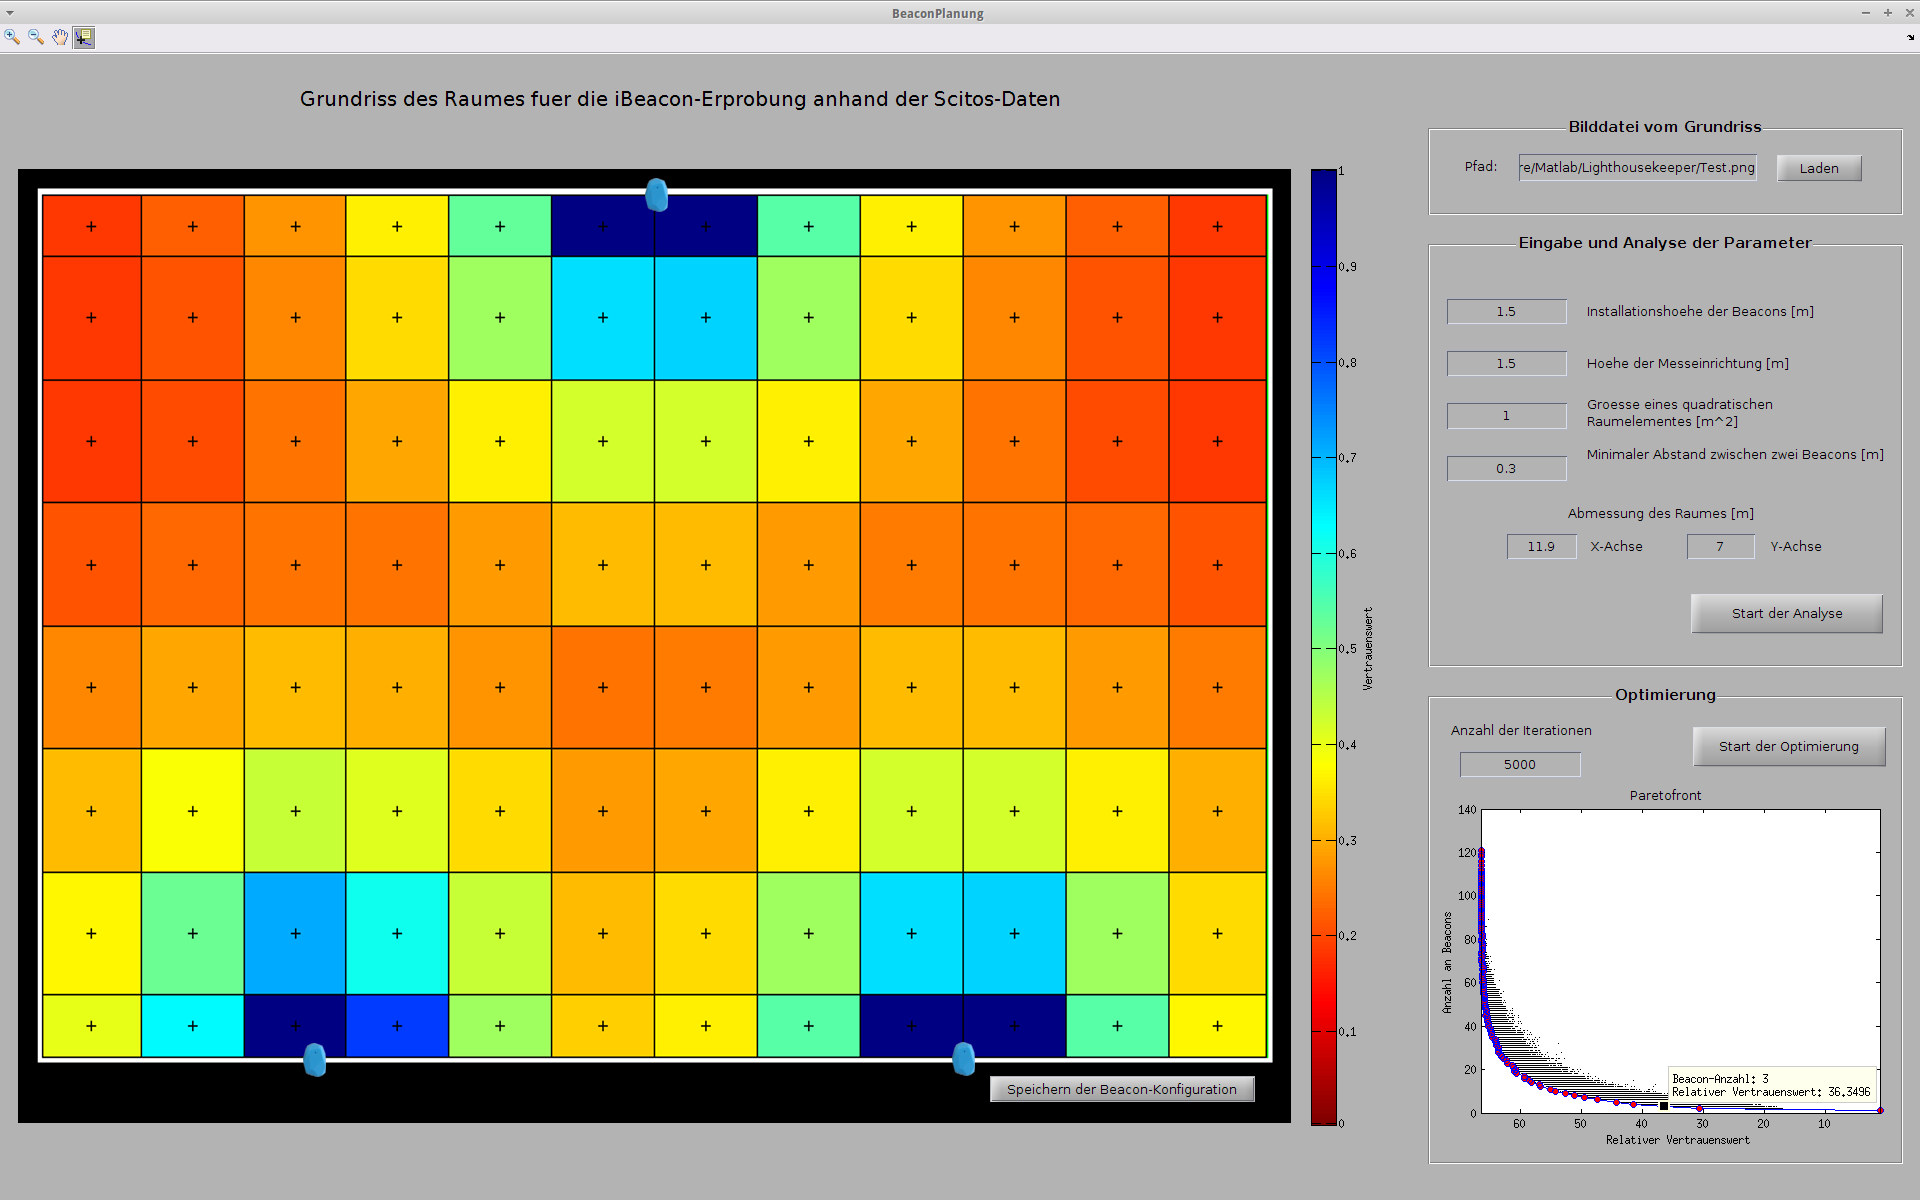
\includegraphics[scale=0.35]{Bilder/Simulationsbeispiel.png}
\caption{Beispiel einer Lighthouse Keeper-Simulation}
\label{fig:Simulationsbeispiel}
\end{figure}
\end{landscape}